\section{Data: Reddit as a community}

We start with a brief overview of both Reddit and the dataset that we use in this paper, focusing on aspects that directly impact our analyses\footnote{There is much more to say about both Reddit itself (see \url{https://www.reddit.com/about/}).}.

\subsection{What is Reddit, briefly}

%% DC 10: Will want a couple of legible screenshots here to help illustrate.
Reddit is one of the largest sharing and discussion communities on the Web.  According to Alexa, as of late 2015 Reddit is in the top 15 sites in the U.S. and the top 35 in the world in terms of monthly unique visitors.  It consists of a large number of subreddits (853 thousand as of June 21st, 2015\footnote{\url{http://www.redditblog.com/2015/06/happy-10th-birthday-to-us-celebrating.html} for more numbers on reddit size.}), each of which focuses on a particular purpose.  Many subreddits are primarily about sharing web content from other sites: in ``Pics'', ``News'', ``Funny'', ``Gaming', and many other communities, users (``Redditors'') make ``submissions'' of links posted at other sites that they think are interesting.  In other subreddits, Redditors primarily write text-based ``self-posts'': ``AskReddit'', ``IamA'', ``ShowerThoughts'' are places where people can ask questions and share stories of their own lives.  Generically, we will refer to submissions and text posts as ``submissions''.  

%% DC 10: Sam should choose a precise terminology here and use it throughout, and be clear on every single analysis exactly what is being counted.  We don't want someone being confused, trying to replicate the data, and finding something different because they don't understand what the analysis is.  (We will also want to be super-clear below when we introduce the dataset to talk about any filtering we did, so that people can exactly replicate what we did.)

%% DC 10: Further, this terminology should agree with Reddit's, so that people who are familiar with the community aren't confused. 

Each post can be imagined as the root of a threaded comment tree; in addition to posting, Redditors can make comments, and vote on both posts and comments.  Votes are used both to sort comments within a post and posts within a subreddit, and also form the basis of ``karma'', a reputation system that essentially tracks how often people upvote a given Redditor's comments and submitted links.  Redditors can also create and volunteer to moderate subreddits.

We choose Reddit as our target community for a number of reasons.  It has existed since 2005, meaning that there has been ample time for the community to evolve and for differences in user cohorts to appear.  Second, being composed of a number of diverse subreddits allows us to explore questions of how communities diverge over time.  Third, Reddit data are publicly available through an API.

\subsection{The dataset}

Redditor \textit{Stuck\_In\_The\_Matrix} used reddit API to compile a dataset of the public available comments \footnote{Available in \url{https://www.reddit.com/r/datasets/comments/3bxlg7/i_have_every_publicly_available_reddit_comment}.} from October 2007 until May 2015. Due to API call failures, he was not able to get about 350 thousand comments. The dataset is composed of 1.65 billion comments. He also compiled a submissions dataset for the period of October 2007 until December 2014, that was made available for us upon request. It contained a total of 114 million submissions.

These datasets contain the JSON data returned by the reddit API. The information in each of these objects \footnote{Full description of the JSON objects in \url{https://github.com/reddit/reddit/wiki/JSON}.} contained the UTC creation date, comment text, author username, subreddit, all relevant information for this work.

%% DC 10: Sam, you gotta fill this out; I don't know the story.

%Amit 9: How was the data made available? Good to explain a little about the source.

We focus on submissions and comments in the dataset because they have timestamps and can be tied to specific users and subreddits, allowing us to perform our time-based analyses.   In some analyses, we look only at comments; in some, we \textbf{combine comments and submissions, calling them ``posts''}.  We would also like to have looked at voting behavior as a measure of user activity\footnote{Which would also give us more insight than usual into lurkers' behavior; we'll return to this in the discussion.}, but individual votes with timestamps and voting user are not available through the API, only the aggregate number of votes that posts receive.
%% DC 10: Adding a note that we know we're ignoring lurkers, both because it's actually important to note that and to avoid being crushed by reviewers who care about lurking.
%%

\subsection{Our processing}

To analyze the data, we used Google BigQuery \footnote{\url{https://cloud.google.com/bigquery/}}, a big data processing tool that allowed us to efficiently navigate within the dataset. The work of importing the comments into BigQuery was done by the redditor \textit{fhoffa}, and the data is publicly available \footnote{More information in \url{https://www.reddit.com/r/bigquery/comments/3cej2b/17_billion_reddit_comments_loaded_on_bigquery/}, users with a Google account can process up to 1TB of data for free in BigQuery by the time this paper was written.}. For the submission data, we uploaded it using Gooogle's SDK \footnote{Part of the alpha code in the SDK, ``gcloud alpha bigquery import''.}.

As our initial pre-processing, we filtered comments and submissions presenting deleted users, data with no creation time and applied a very simple bot removal. The SQL constraints are shown below.

\begin{verbatim}
created_utc is not NULL
and author <> '[deleted]'
and not right(author, 4) = '_bot'
and not right(author, 3) = 'Bot'
and not lower(author) contains 'transcriber'
and not lower(author) contains 'automoderator'
\end{verbatim}

We also considered only comment data from October 2007 until December 2014 in order to have a matching period for comments and submissions. After this process, we had a total of 1.17 billion comments and 114 million submissions.

%% DC 10: Can we also please get rid of 2007 in all the figures?  It appears that 
\subsection{An overview of the dataset}

%% DC 10: Assuming because you say comment you really mean "comments".  That's fine (though I wonder if it would make more sense in the overview for both this and for active to combine both posts and comments as "activity")

%% DC 10: Unless the ratio has useful analysis to be done, we should get rid of it as noise.

%% DC 10: I tike that the figure axes are much more legible.  But, things still to fix: Axes should be meaningful labels: "Average posts per user". "Total Created".  "Total Active Per Month".  Figures should have legend items in the same vertical order as data series, and the series should also probably be drawn not just with colors but with different patterns, to faciliate their reading in black and white.  Charts with a single data series probably don't need a legend (which should just be embedded in the caption).  This should get fixed throughout once we've decided exactly which figures to keep.
\begin{figure*}[!tb]
\centering
\begin{subfigure}{.49\textwidth}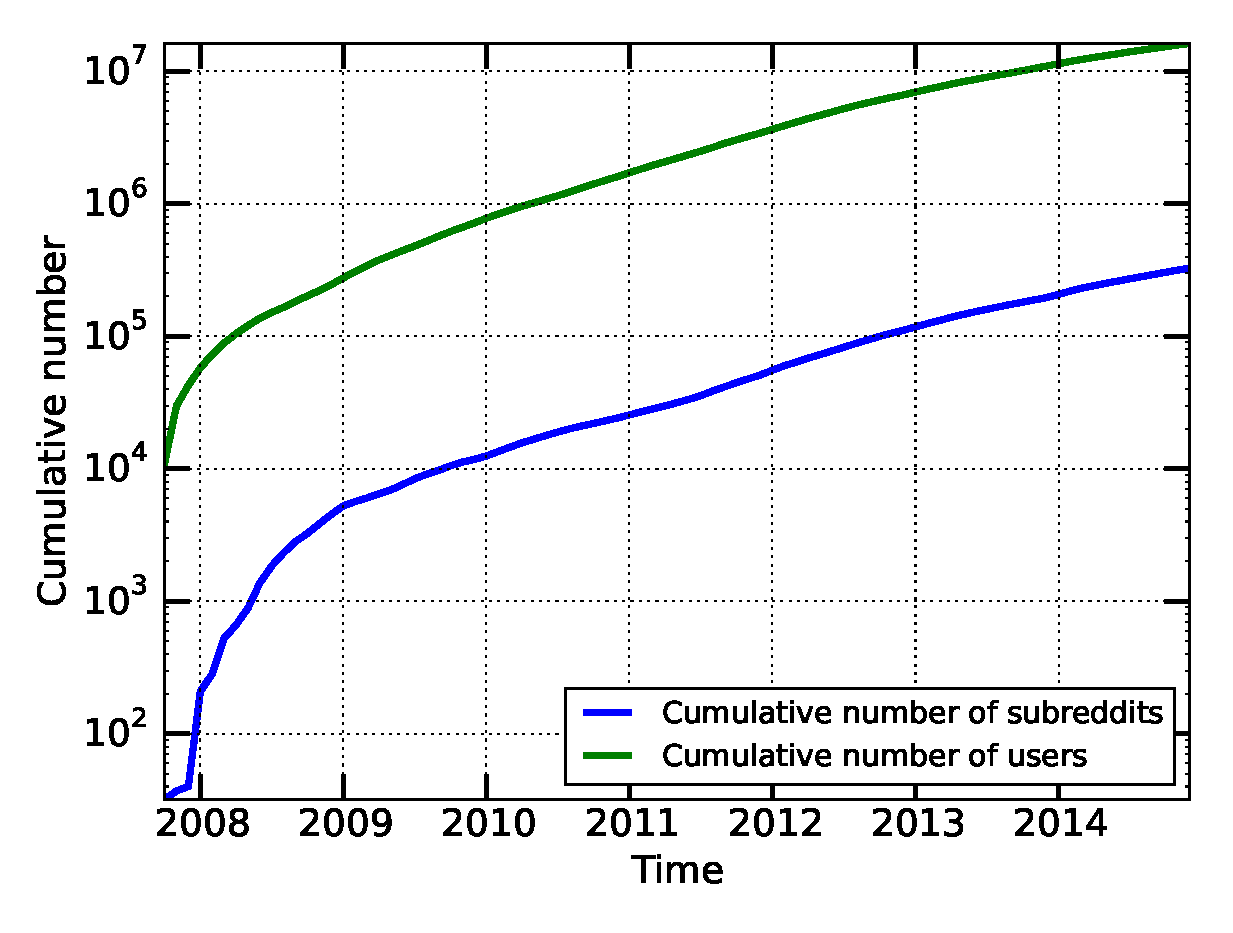
\includegraphics[scale=0.4]{./images/cumulative_users_subreddits.eps}\caption{}\end{subfigure}
\begin{subfigure}{.49\textwidth}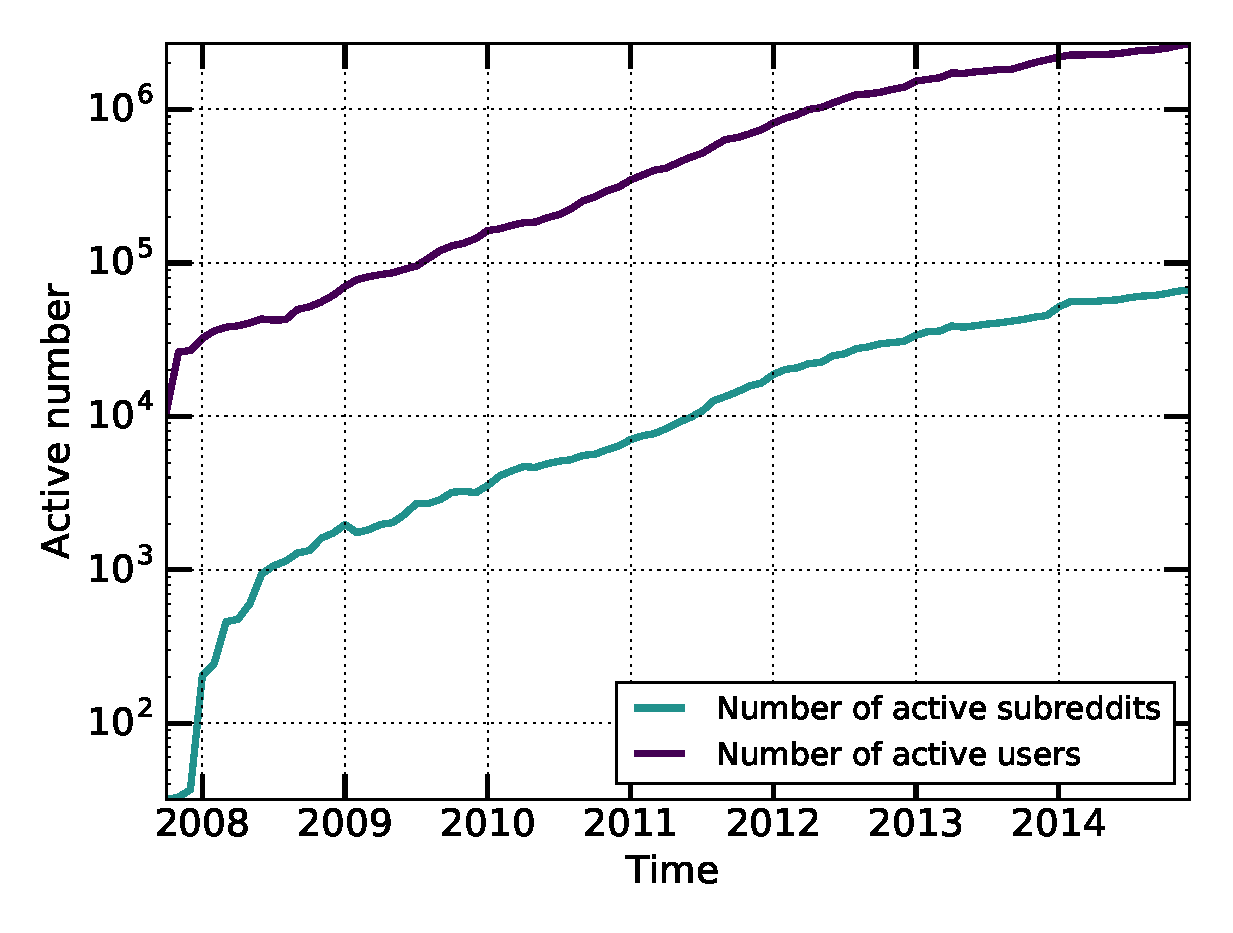
\includegraphics[scale=0.4]{./images/active_users_subreddits.eps}\caption{}\end{subfigure}
\caption{Figure a shows the cumulative growth of reddit for users and subreddits. Figure b shows the number of active users and subreddits in reddit over time. An active user or subreddit is the one that presented at least one post (comment or submission) in the time bin we used --- time here is discretized by month.}
\label{fig:cumulative}
\end{figure*}

% DC 10: Aga
%Figures~\ref{fig:cumulative_users_subreddits}~and~\ref{fig:active_users_subreddits} show an overview of Reddit's growth over time.  
%% Sam 12: Will remove the ratio line since we don't particularly user it for any analysis.
Here we present an overview of reddit and how it grew in the past few years. Figure~\ref{fig:cumulative}a shows the cumulative number of user accounts and subreddits created over time as of the last day of every month. After an initial extremely rapid expansion from 2008--2009, both the number of users and subreddits have grown exponentially.  As of the end of 2014, about 16.2 million distinct users have made at least one comment and 327 thousand subreddits received at least one comment since Reddit's inception.

%% DC 10: Since there can be redditors that only submit and don't comment, if this is really comments then it understates activity -- so I am now even more convinced that this should be combined submissions and comments.
%% Sam 10: The active subreddits and user accounts are all based on the joint submission and comment behavior.
However, as with many other online sites, most users \cite{} and communities \cite{butler_kraut_paper} do not stay active. Figure~\ref{fig:cumulative}b shows the monthly number of user accounts and subreddits that made or received at least one post (our definition of post is either a comment or a submission). We define as an \textbf{active user the one that made at least one post in the month} in question. Similarly, an \textbf{active subreddit is the one that received at least one post in the month}. In December 2014, about 470,000 thousand users made posts and about 11,400 subreddits received posts; both are an order of magnitude less than the cumulative number of users or subreddits.  

%\begin{figure}[!tb]
%\centering
%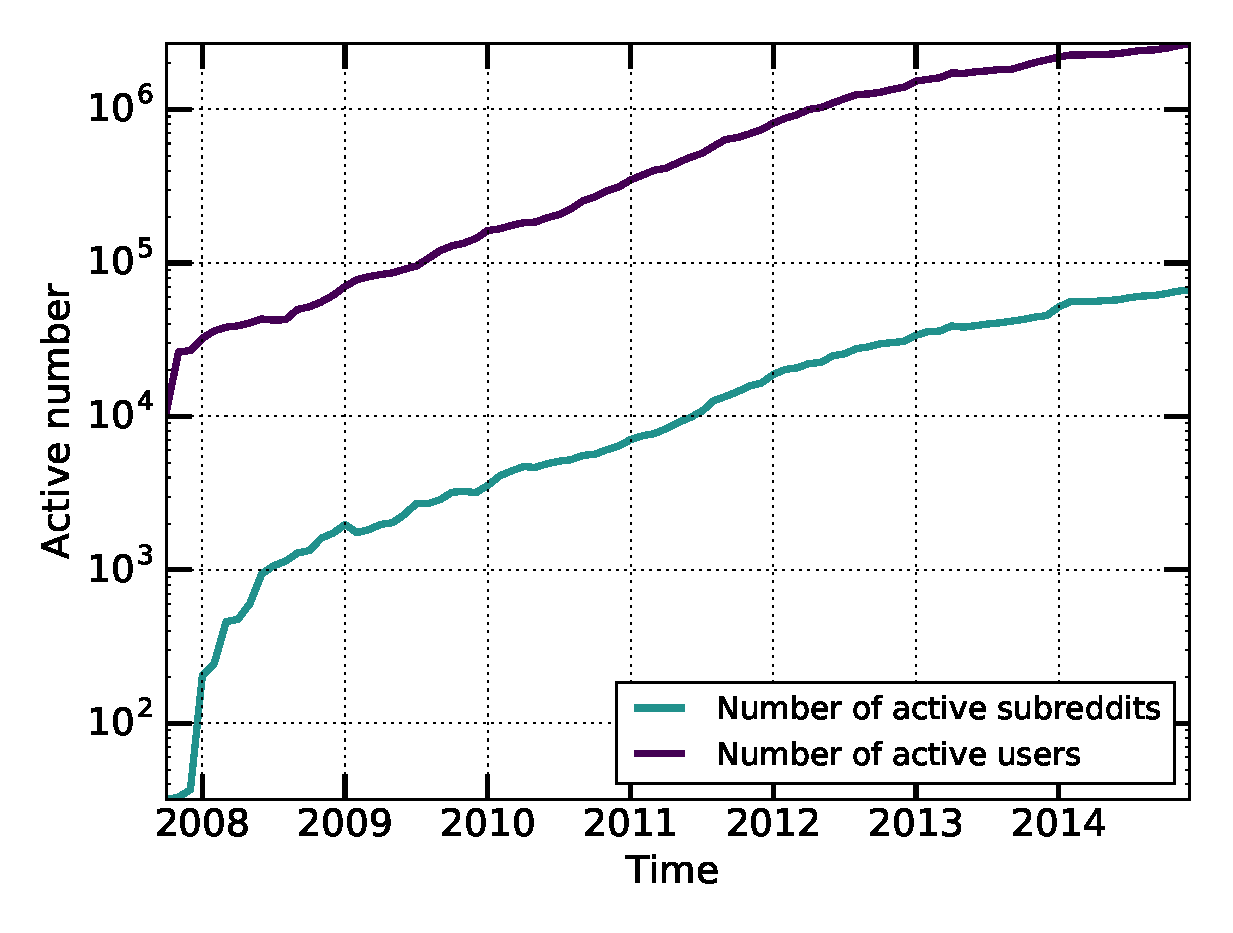
\includegraphics[scale=0.4]{./images/active_users_subreddits.eps}
%\caption{Number of active users and subreddits in reddit over time. An active user or subreddit is the one that presented at least one post in the time bin we used --- time here is discretized by month.}
%\label{fig:active_users_subreddits}
%\end{figure}

The fact that such a significant amount of users stopped using the platform raises questions such as why users give up on their accounts, when they do so, and which users are more likely to stay active. In later sections we will take a closer look at how some of these things are happening in reddit.

\subsection{Identifying cohorts}
%% DC 10: Trying to decide whether this works better here or at the beginning of a cohorty section -- there is some subtlety that I think Sam wants to work through when introducing the first problem.
%% Amit 9: Added this subsection here. Having the cohorts defined as the part of the overview will help, as we talk about them throughout the paper. Some of the cohort stuff from next section can come here. 

As we defined before, the account creation time is the time of the first post the user created. Similarly, the subreddit creation time is the time of the first post that it received. Throughout this paper, we will use the notion of user (subreddits) cohorts, which will consist of users (subreddits) with the same creation year.

In many cases, we will look at the time evolution of these cohorts. Since users (subreddits) can be created in the beggining of the referred year or in the end and our dataset has a date limit threshold, we are likely to have a variation on the data available for each user of up to one year, even though they are in the same cohort. To deal with this, many of our cohorted analysis will consider only the overlapping time window for which we collect data for all users. This means that we are going to cut one year at the end of some analysis to guarantee that we are not biased by users created early or later inside of the cohort.

Our data also starts in October 2007, but reddit has existed before it. That means that, not only we have incomplete data for the 2007 year (which compromises this cohort), but also there might be users and subreddits that show up in 2007 that were actually created in the previous years. Since we can not control for these, we will also omit 2007 cohort, for it is not representative of 2007. We will, however, include 2007 in the overall analysis over time (the non cohorted ones) for two reasons: first, it does not have any direct impact in the results, only extends the axis for 3 extra months and secondly, we often compare the cohorted approach with a simple, naive approach, and we would not expect a naive approach to do any kind of filtering.